\documentclass[showpacs, preprintnumbers, pra, superscriptaddress, floatfix, onecolumn, longbibliography]{revtex4-1}
\usepackage{amssymb}
\usepackage{amsmath}
\usepackage{float}
\usepackage{graphicx}
\usepackage{epsfig}
\usepackage[T1]{fontenc}
\usepackage{color}


\usepackage[utf8]{inputenc}
%\topmargin=0.2cm

\newcommand{\beq}{\begin{equation}}
\newcommand{\eeq}{\end{equation}}
\newcommand{\bea}{\begin{eqnarray}}
\newcommand{\eea}{\end{eqnarray}}
\newcommand{\nn}{\nonumber}
\newcommand{\no}{\noindent}
\newcommand{\hs}{\hspace{0.1cm}}
\newcommand{\spz}{\hspace{0.7cm}}
\newcommand{\st}{\stackrel}
\newcommand{\eps}{\epsilon}
\newcommand{\veps}{\varepsilon}
\newcommand{\al}{\alpha}
\newcommand{\s}{\sigma}
\newcommand{\lam}{\lambda}
\newcommand{\om}{\omega}
\newcommand{\iom}{i\omega_n}
\newcommand{\de}{\delta}
\newcommand{\D}{\Delta}
\newcommand{\goto}{\rightarrow}
\newcommand{\lab}{\label}
\newcommand{\be}{\beta}
\newcommand{\zb}{\bar{z}}
\newcommand{\p}{\partial}\newcommand{\vp}{\varphi}
\newcommand{\ra}{\rangle}
\newcommand{\la}{\langle}
\newcommand{\Ga}{\Gamma}
\newcommand{\ga}{\gamma}
\newcommand{\app}{\approx}
\newcommand{\ua}{\uparrow}
\newcommand{\da}{\downarrow}
\newcommand{\Ua}{\Uparrow}
\newcommand{\Da}{\Downarrow}
\newcommand{\dmi}{\frac{1}{2}}
\newcommand{\lra}{\longrightarrow}
\newcommand{\Lra}{\Leftrightarrow}
\newcommand{\tht}{\theta}
\newcommand{\pbf}{}
\newcommand{\SM}{S}
\newcommand{\uul}[1] {\underline{\underline{ #1}}}
\def\mean#1{\left< #1 \right>}

\begin{document}

\title{}


\maketitle

\section{Details of the density-functional (DFT) calculations}

All DFT-based results of this work are obtained with a calculation of a MnBi$_4$Te$_7$ slab made of eight structural blocks (i.e. four septuple layers and four quintuple layers) and of a vacuum of 30 Bohr and based on experimental lattice parameters (Fig. \ref{dft_structure}a)).
We use the LSDA+U method with the generalized grandient approximation as implemented in the FPLO method \cite{}. We fix parameters $U=5.34\,$eV and $J=0$, as in Ref. \cite{}. The spin-orbit interaction is considered in the fully-relativistic four-component formalism. Numerial integrations are performed with a tetrahedron method with a mesh of $12\times12\times1$ subdivisions in the Brillouin zone.

For the simulation of the orbital-projected surface spectral density in Fig. 3 of the main text, we take into account all Bloch states in the slab, weighting their contribution with an exponential decaying factor (Fig. \ref{dft_structure}b). Specifically, denoting the local orbitals as $|\phi^{(z)}_{jm}\rangle$, where $z$ is the distance from the orbital to the surface, for each Bloch state $|\psi_{k_0\nu}\rangle$ of energy $\varepsilon_{k_0\nu}$, we consider as its contribution 
\begin{equation}
A_{jm}(\omega,k)=\frac{1}{\pi}\frac{ \Delta_\varepsilon}{(\omega-\varepsilon_{k\nu})^2 + \Delta^2_\varepsilon}\frac{ \Delta_k}{(k-k_0)^2 + \Delta^2_k }|\langle \phi^{(z)}_{jm} | \psi_{k_0\nu} \rangle|^2 \text{e}^{-z/\lambda},
\end{equation}
where $\lambda=10\,$\AA, $\Delta_\varepsilon=20\,$meV and $\Delta_k=0.005$\AA$^{-1}$. Last, notice that the local orbitals in Fig. 3 of the main text are defined with the cartesian coordinate system shown in Fig. \ref{dft_structure}c).

\begin{figure*}[h!]
 \centering
 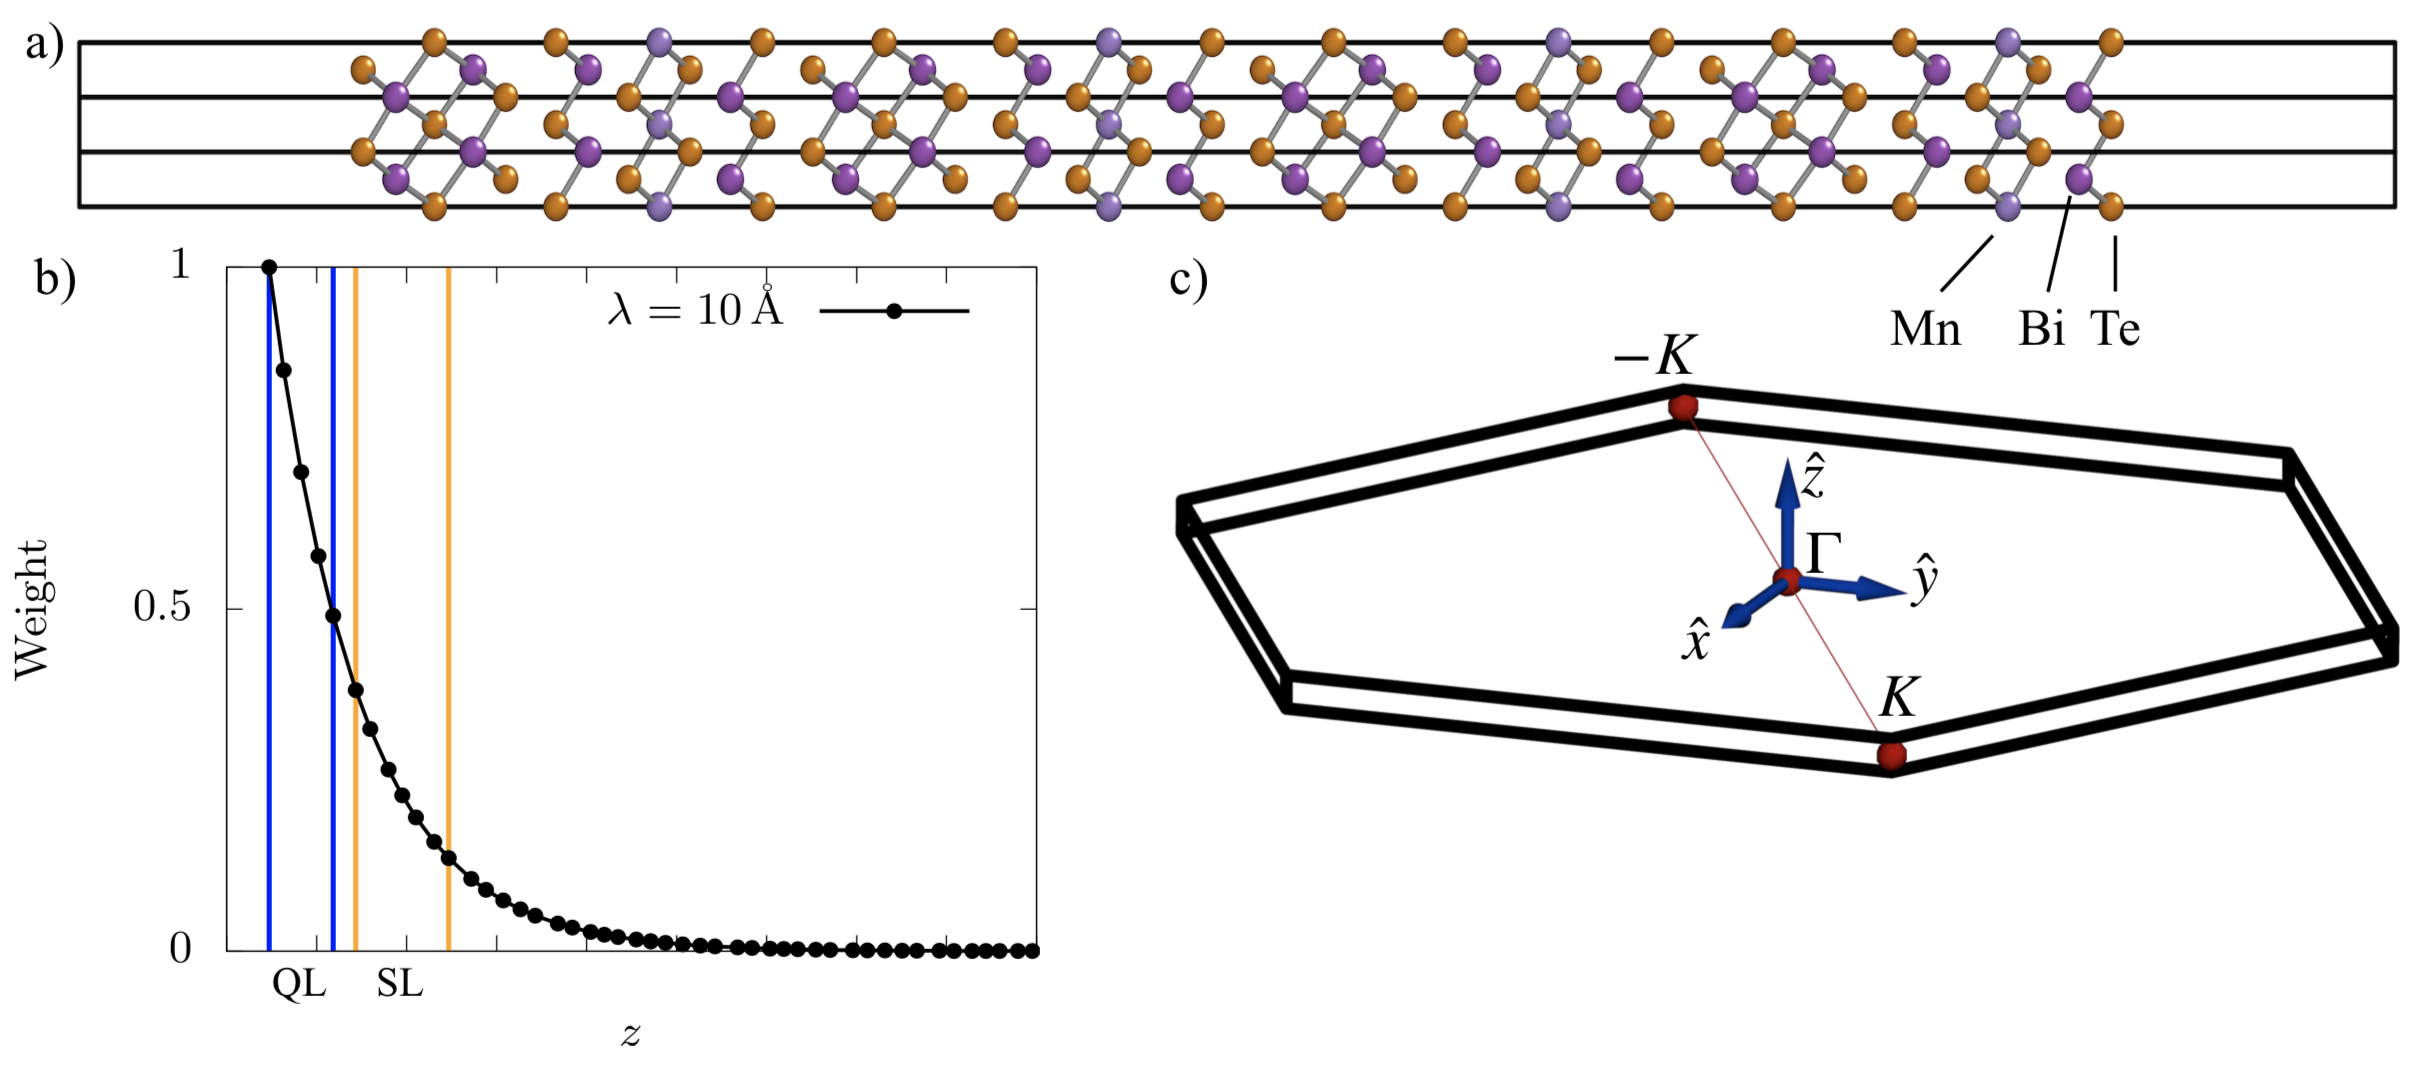
\includegraphics[width=14 cm]{structural_data.png}
	\caption{a) Structural model used in the density-functional calculation. b) Illustration of the exponential decaying weight considered for the surface spectral weight simulation. c) Brillouin zone.} 
	\label{dft_structure}
\end{figure*}

\section{Surface density of states}
\begin{figure*}[h!]
 \centering
 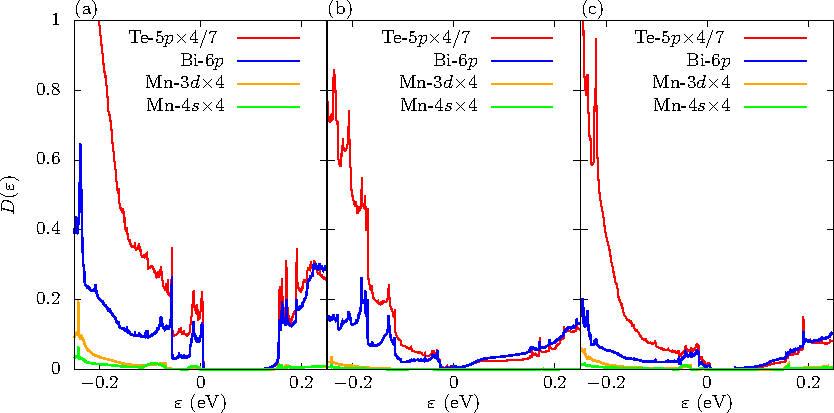
\includegraphics[width=15 cm]{dos.pdf}
	\caption{ Bulk density of states (a) and surface density of states for the quintuple layer (b) and septuple layer (c) terminations. For the bulk, we consider the total density of states of the slab projected on the quintuple and septuple layer in the center of the slab. 	}
	\label{dft_sl}
\end{figure*}



\section{Surface state angular momentum reversal within DFT}
Fig. \ref{dft_sl} illustrates the angular momentum reversal between the upper and lower parts of the surface state, as obtained with DFT. 
Fig. \ref{dft_sl}a) presents the band-structure projected on the outmost septuple layer and Fig. \ref{dft_sl}b) shows constant-energy contours. The color-scale reflects the amplitud of the corresponding states on local orbitals of Bi or Te and $J=1/2$, which we found dominate the upper part of the Dirac cone.
Notice that since the experiment of natural dichroism described in the main text is essentially susceptible to the in-plane angular momentum, in this figure the fully relativistic local orbitals considered are defined with the quantization axis along the in-plane cartesian direction $\hat{x}$.
\begin{figure*}[h!]
 \centering
 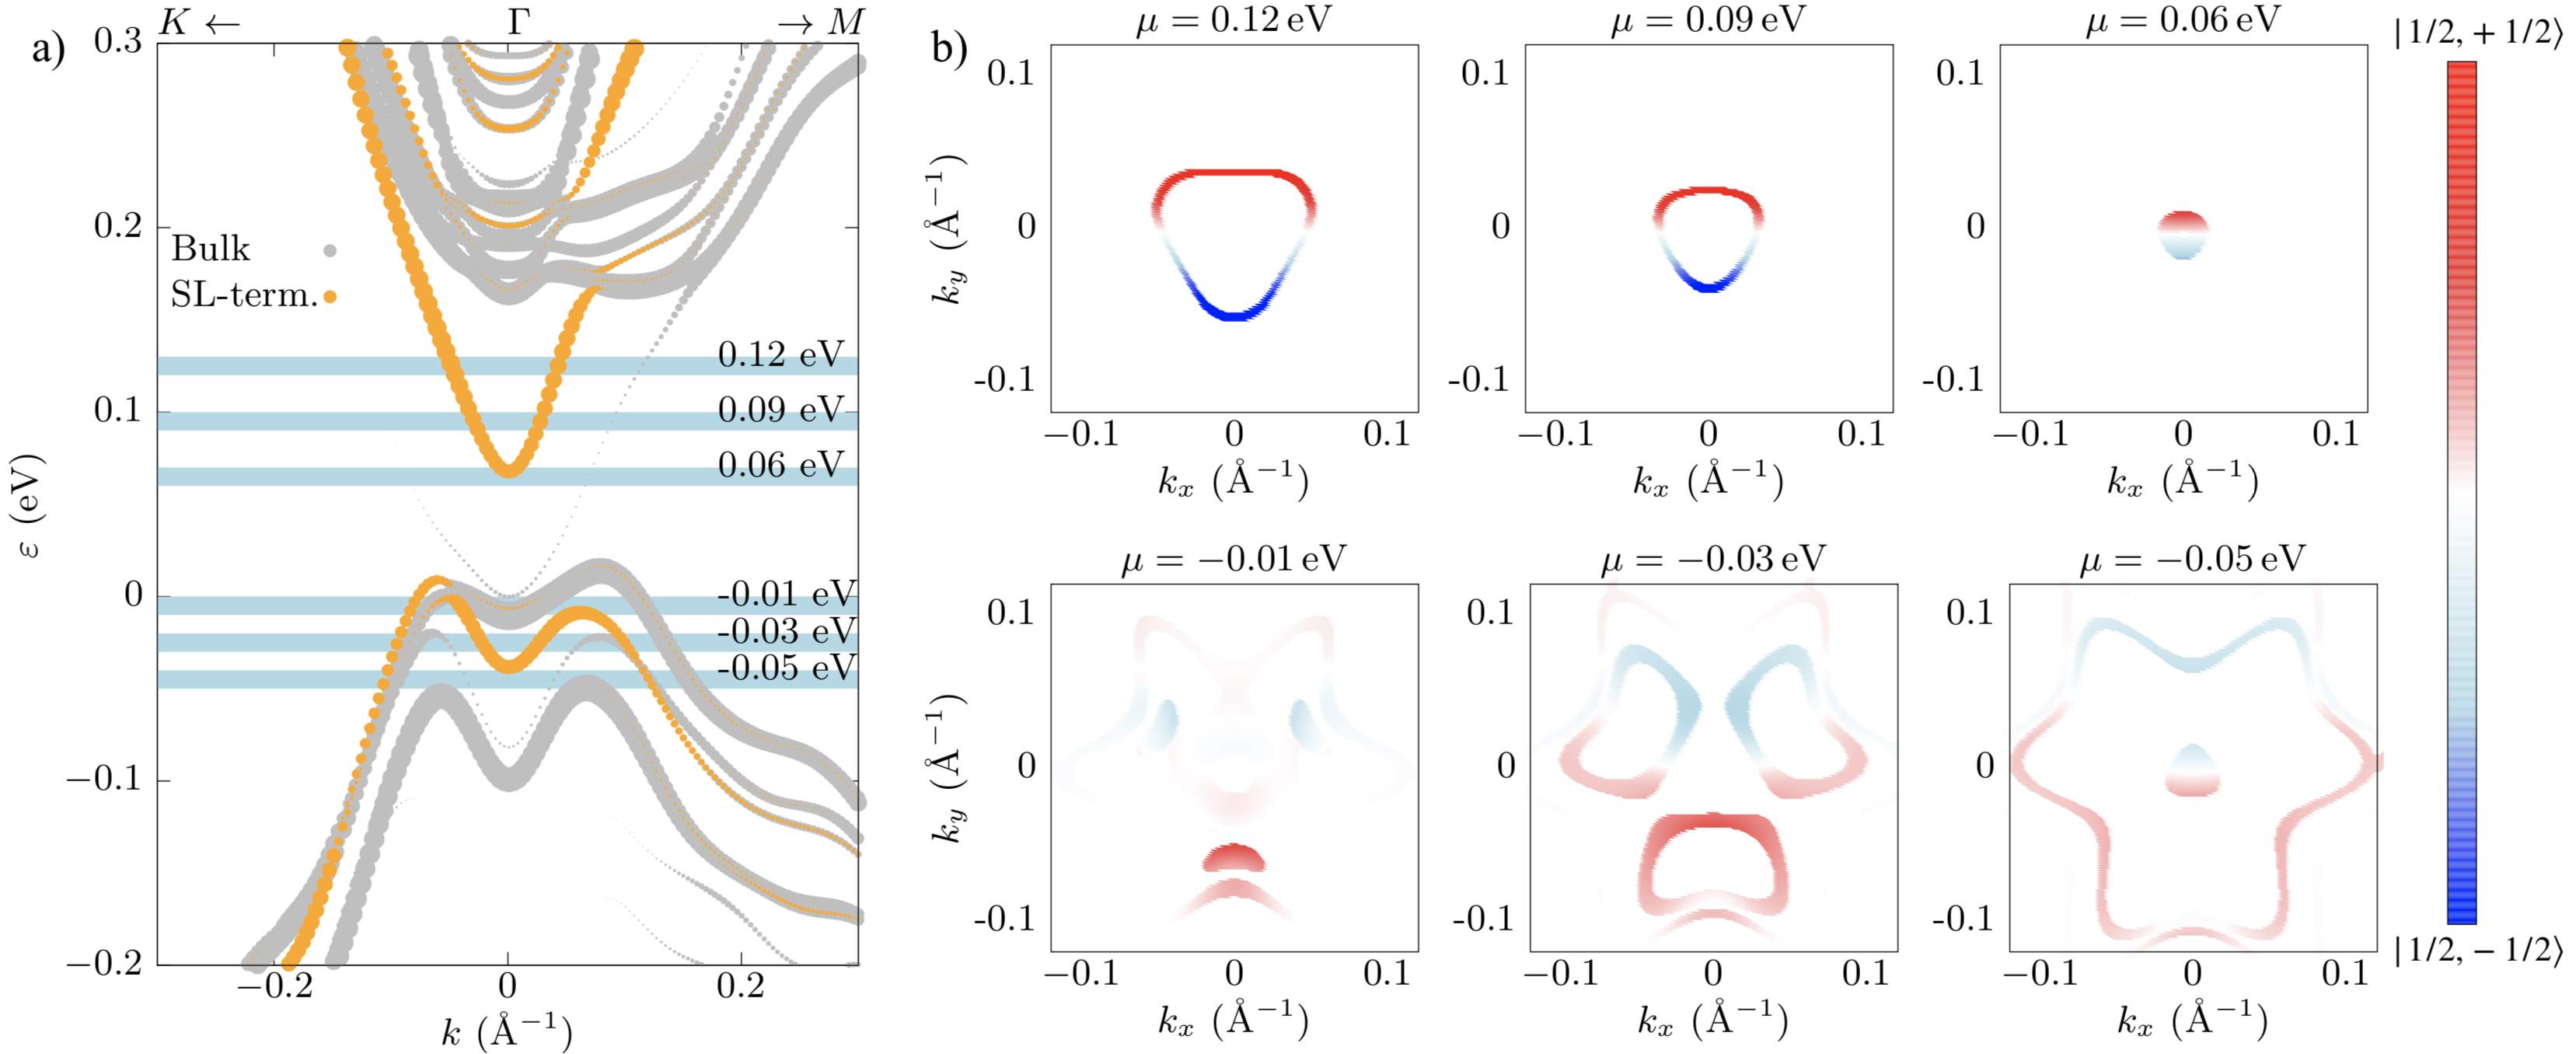
\includegraphics[width=18 cm]{sl.png}
	\caption{a) MnBi$_4$Te$_7$ band structure projected on the outmost septuple layer (SL-term.) and on the four inner blocks (Bulk). 
	b): Constant energy contours of septuple layer-projected band-structure. In this projection, for simplicity we only consider the Bi or Te states with $J=1/2$, which we found to dominate the upper part of the Dirac cone.
	}
	\label{dft_sl}
\end{figure*}


\bibliography{ref}
\end{document}


